\documentclass{standalone}
\usepackage{tikz}
\usetikzlibrary{patterns, positioning}

\begin{document}
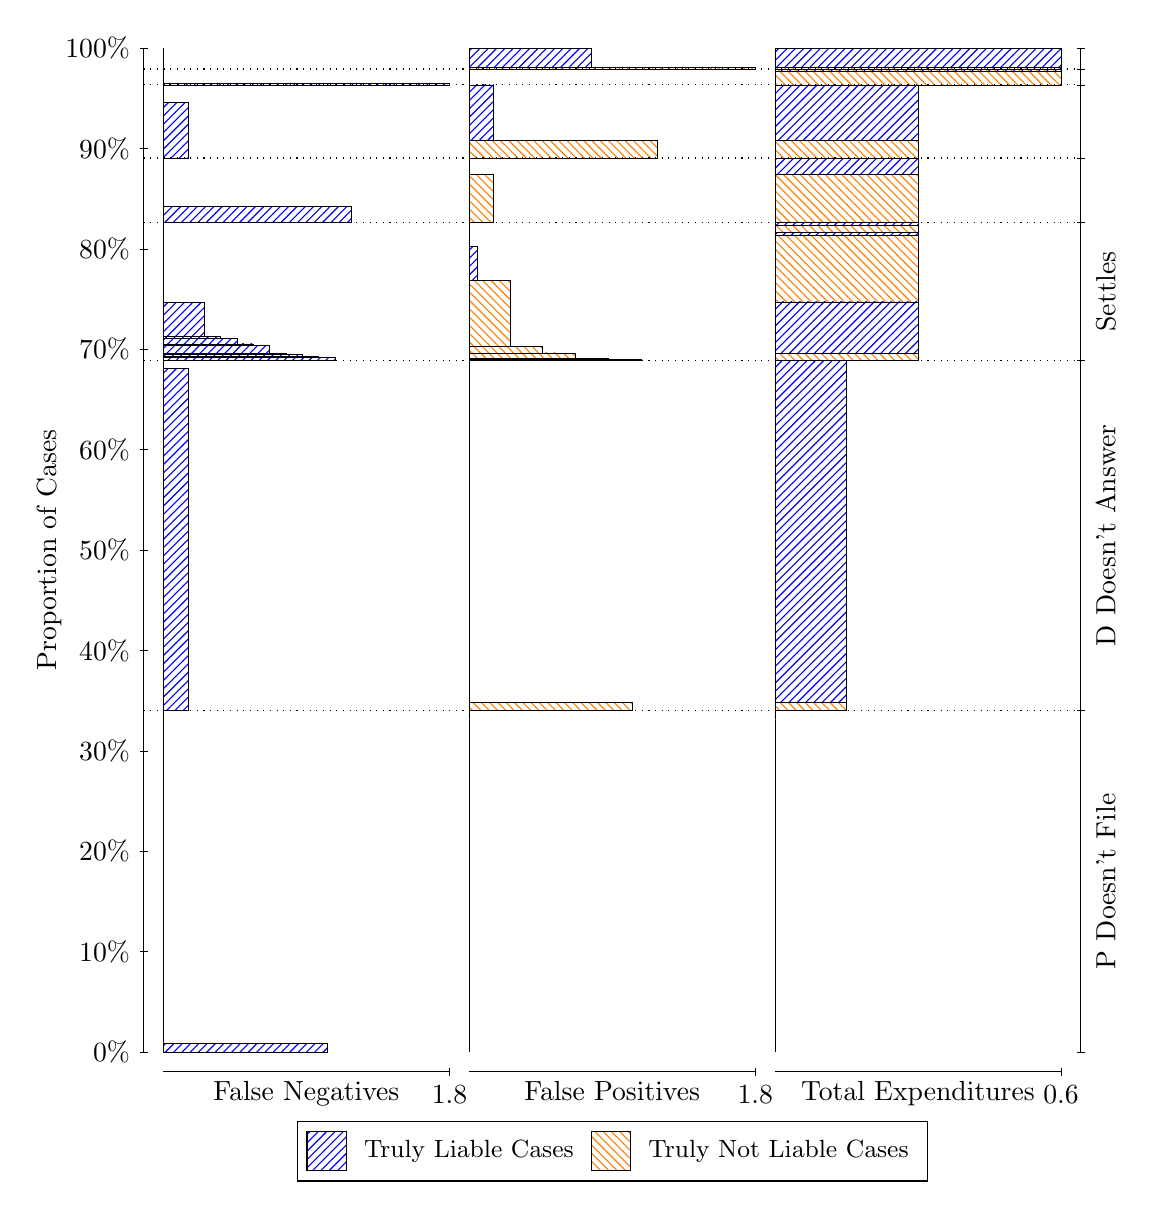
\begin{tikzpicture}
\draw[black, very thin] (1.5,1.75) -- (1.5,14.5);
\node[rotate=90, anchor=center] at (0.3, 8.125) {Proportion of Cases};
\draw[black, very thin] (1.45,1.75) -- (1.55,1.75);
\node[anchor=east] at (1.45, 1.75) {0\%};
\draw[black, very thin] (1.45,3.025) -- (1.55,3.025);
\node[anchor=east] at (1.45, 3.025) {10\%};
\draw[black, very thin] (1.45,4.3) -- (1.55,4.3);
\node[anchor=east] at (1.45, 4.3) {20\%};
\draw[black, very thin] (1.45,5.575) -- (1.55,5.575);
\node[anchor=east] at (1.45, 5.575) {30\%};
\draw[black, very thin] (1.45,6.85) -- (1.55,6.85);
\node[anchor=east] at (1.45, 6.85) {40\%};
\draw[black, very thin] (1.45,8.125) -- (1.55,8.125);
\node[anchor=east] at (1.45, 8.125) {50\%};
\draw[black, very thin] (1.45,9.4) -- (1.55,9.4);
\node[anchor=east] at (1.45, 9.4) {60\%};
\draw[black, very thin] (1.45,10.675) -- (1.55,10.675);
\node[anchor=east] at (1.45, 10.675) {70\%};
\draw[black, very thin] (1.45,11.95) -- (1.55,11.95);
\node[anchor=east] at (1.45, 11.95) {80\%};
\draw[black, very thin] (1.45,13.225) -- (1.55,13.225);
\node[anchor=east] at (1.45, 13.225) {90\%};
\draw[black, very thin] (1.45,14.5) -- (1.55,14.5);
\node[anchor=east] at (1.45, 14.5) {100\%};

\draw[black, very thin] (13.4,1.75) -- (13.4,14.5);
\draw[black, very thin] (13.35,1.75) -- (13.45,1.75);
\node[anchor=west] at (13.35, 1.75) {};
\draw[black, very thin] (13.35,6.0872) -- (13.45,6.0872);
\node[anchor=west] at (13.35, 6.0872) {};
\draw[black, very thin] (13.35,10.533) -- (13.45,10.533);
\node[anchor=west] at (13.35, 10.533) {};
\draw[black, very thin] (13.35,12.287) -- (13.45,12.287);
\node[anchor=west] at (13.35, 12.287) {};
\draw[black, very thin] (13.35,13.103) -- (13.45,13.103);
\node[anchor=west] at (13.35, 13.103) {};
\draw[black, very thin] (13.35,14.032) -- (13.45,14.032);
\node[anchor=west] at (13.35, 14.032) {};
\draw[black, very thin] (13.35,14.233) -- (13.45,14.233);
\node[anchor=west] at (13.35, 14.233) {};
\draw[black, very thin] (13.35,14.5) -- (13.45,14.5);
\node[anchor=west] at (13.35, 14.5) {};

\draw[black, very thin, pattern color=blue, pattern=north east lines] (1.75,1.75) rectangle (3.8262,1.8637);
\draw[black, very thin, pattern color=orange, pattern=north west lines] (1.75,1.8637) rectangle (1.75,6.0872);
\draw[black, very thin, pattern color=blue, pattern=north east lines] (1.75,6.0872) rectangle (2.0614,10.432);
\draw[black, very thin, pattern color=orange, pattern=north west lines] (1.75,10.432) rectangle (1.75,10.533);
\draw[black, very thin, pattern color=blue, pattern=north east lines] (1.75,10.533) rectangle (3.93,10.575);
\draw[black, very thin, pattern color=blue, pattern=north east lines] (1.75,10.575) rectangle (3.7224,10.58);
\draw[black, very thin, pattern color=blue, pattern=north east lines] (1.75,10.58) rectangle (3.5148,10.612);
\draw[black, very thin, pattern color=blue, pattern=north east lines] (1.75,10.612) rectangle (3.3071,10.623);
\draw[black, very thin, pattern color=blue, pattern=north east lines] (1.75,10.623) rectangle (3.0995,10.725);
\draw[black, very thin, pattern color=blue, pattern=north east lines] (1.75,10.725) rectangle (2.8919,10.744);
\draw[black, very thin, pattern color=blue, pattern=north east lines] (1.75,10.744) rectangle (2.6843,10.817);
\draw[black, very thin, pattern color=blue, pattern=north east lines] (1.75,10.817) rectangle (2.4767,10.841);
\draw[black, very thin, pattern color=blue, pattern=north east lines] (1.75,10.841) rectangle (2.269,11.267);
\draw[black, very thin, pattern color=orange, pattern=north west lines] (1.75,11.267) rectangle (1.75,12.287);
\draw[black, very thin, pattern color=blue, pattern=north east lines] (1.75,12.287) rectangle (4.1376,12.491);
\draw[black, very thin, pattern color=orange, pattern=north west lines] (1.75,12.491) rectangle (1.75,13.103);
\draw[black, very thin, pattern color=blue, pattern=north east lines] (1.75,13.103) rectangle (2.0614,13.81);
\draw[black, very thin, pattern color=orange, pattern=north west lines] (1.75,13.81) rectangle (1.75,14.032);
\draw[black, very thin, pattern color=blue, pattern=north east lines] (1.75,14.032) rectangle (5.3833,14.054);
\draw[black, very thin, pattern color=orange, pattern=north west lines] (1.75,14.054) rectangle (1.75,14.233);
\draw[black, very thin, pattern color=orange, pattern=north west lines] (1.75,14.233) rectangle (1.75,14.252);
\draw[black, very thin, pattern color=blue, pattern=north east lines] (1.75,14.252) rectangle (1.75,14.5);
\draw[black, very thin, pattern color=orange, pattern=north west lines] (5.6333,1.75) rectangle (5.6333,5.9734);
\draw[black, very thin, pattern color=blue, pattern=north east lines] (5.6333,5.9734) rectangle (5.6333,6.0872);
\draw[black, very thin, pattern color=orange, pattern=north west lines] (5.6333,6.0872) rectangle (7.7095,6.1883);
\draw[black, very thin, pattern color=blue, pattern=north east lines] (5.6333,6.1883) rectangle (5.6333,10.533);
\draw[black, very thin, pattern color=orange, pattern=north west lines] (5.6333,10.533) rectangle (7.8133,10.543);
\draw[black, very thin, pattern color=orange, pattern=north west lines] (5.6333,10.543) rectangle (7.6057,10.546);
\draw[black, very thin, pattern color=orange, pattern=north west lines] (5.6333,10.546) rectangle (7.3981,10.556);
\draw[black, very thin, pattern color=orange, pattern=north west lines] (5.6333,10.556) rectangle (7.1905,10.559);
\draw[black, very thin, pattern color=orange, pattern=north west lines] (5.6333,10.559) rectangle (6.9829,10.62);
\draw[black, very thin, pattern color=orange, pattern=north west lines] (5.6333,10.62) rectangle (6.7752,10.626);
\draw[black, very thin, pattern color=orange, pattern=north west lines] (5.6333,10.626) rectangle (6.7752,10.629);
\draw[black, very thin, pattern color=orange, pattern=north west lines] (5.6333,10.629) rectangle (6.5676,10.709);
\draw[black, very thin, pattern color=orange, pattern=north west lines] (5.6333,10.709) rectangle (6.36,10.712);
\draw[black, very thin, pattern color=orange, pattern=north west lines] (5.6333,10.712) rectangle (6.1524,11.553);
\draw[black, very thin, pattern color=blue, pattern=north east lines] (5.6333,11.553) rectangle (5.7371,11.979);
\draw[black, very thin, pattern color=blue, pattern=north east lines] (5.6333,11.979) rectangle (5.6333,12.287);
\draw[black, very thin, pattern color=orange, pattern=north west lines] (5.6333,12.287) rectangle (5.9448,12.898);
\draw[black, very thin, pattern color=blue, pattern=north east lines] (5.6333,12.898) rectangle (5.6333,13.103);
\draw[black, very thin, pattern color=orange, pattern=north west lines] (5.6333,13.103) rectangle (8.021,13.325);
\draw[black, very thin, pattern color=blue, pattern=north east lines] (5.6333,13.325) rectangle (5.9448,14.032);
\draw[black, very thin, pattern color=orange, pattern=north west lines] (5.6333,14.032) rectangle (5.6333,14.21);
\draw[black, very thin, pattern color=blue, pattern=north east lines] (5.6333,14.21) rectangle (5.6333,14.233);
\draw[black, very thin, pattern color=orange, pattern=north west lines] (5.6333,14.233) rectangle (9.2667,14.252);
\draw[black, very thin, pattern color=blue, pattern=north east lines] (5.6333,14.252) rectangle (7.1905,14.5);
\draw[black, very thin, pattern color=orange, pattern=north west lines] (9.5167,1.75) rectangle (9.5167,5.9734);
\draw[black, very thin, pattern color=blue, pattern=north east lines] (9.5167,5.9734) rectangle (9.5167,6.0872);
\draw[black, very thin, pattern color=orange, pattern=north west lines] (9.5167,6.0872) rectangle (10.425,6.1883);
\draw[black, very thin, pattern color=blue, pattern=north east lines] (9.5167,6.1883) rectangle (10.425,10.533);
\draw[black, very thin, pattern color=orange, pattern=north west lines] (9.5167,10.533) rectangle (11.333,10.626);
\draw[black, very thin, pattern color=blue, pattern=north east lines] (9.5167,10.626) rectangle (11.333,11.276);
\draw[black, very thin, pattern color=orange, pattern=north west lines] (9.5167,11.276) rectangle (11.333,12.117);
\draw[black, very thin, pattern color=blue, pattern=north east lines] (9.5167,12.117) rectangle (11.333,12.159);
\draw[black, very thin, pattern color=orange, pattern=north west lines] (9.5167,12.159) rectangle (11.333,12.245);
\draw[black, very thin, pattern color=blue, pattern=north east lines] (9.5167,12.245) rectangle (11.333,12.287);
\draw[black, very thin, pattern color=orange, pattern=north west lines] (9.5167,12.287) rectangle (11.333,12.898);
\draw[black, very thin, pattern color=blue, pattern=north east lines] (9.5167,12.898) rectangle (11.333,13.103);
\draw[black, very thin, pattern color=orange, pattern=north west lines] (9.5167,13.103) rectangle (11.333,13.325);
\draw[black, very thin, pattern color=blue, pattern=north east lines] (9.5167,13.325) rectangle (11.333,14.032);
\draw[black, very thin, pattern color=orange, pattern=north west lines] (9.5167,14.032) rectangle (13.15,14.21);
\draw[black, very thin, pattern color=blue, pattern=north east lines] (9.5167,14.21) rectangle (13.15,14.233);
\draw[black, very thin, pattern color=orange, pattern=north west lines] (9.5167,14.233) rectangle (13.15,14.252);
\draw[black, very thin, pattern color=blue, pattern=north east lines] (9.5167,14.252) rectangle (13.15,14.5);
\draw[black, dotted] (1.5,6.0872) -- (13.4,6.0872);
\draw[black, dotted] (1.5,10.533) -- (13.4,10.533);
\draw[black, dotted] (1.5,12.287) -- (13.4,12.287);
\draw[black, dotted] (1.5,13.103) -- (13.4,13.103);
\draw[black, dotted] (1.5,14.032) -- (13.4,14.032);
\draw[black, dotted] (1.5,14.233) -- (13.4,14.233);
\draw[black, very thin] (1.75,1.5) -- (5.3833,1.5);
\node[anchor=north] at (3.5667, 1.5) {False Negatives};
\draw[black, very thin] (5.3833,1.45) -- (5.3833,1.55);
\node[anchor=north] at (5.3833, 1.45) {1.8};

\draw[black, very thin] (5.6333,1.5) -- (9.2667,1.5);
\node[anchor=north] at (7.45, 1.5) {False Positives};
\draw[black, very thin] (9.2667,1.45) -- (9.2667,1.55);
\node[anchor=north] at (9.2667, 1.45) {1.8};

\draw[black, very thin] (9.5167,1.5) -- (13.15,1.5);
\node[anchor=north] at (11.333, 1.5) {Total Expenditures};
\draw[black, very thin] (13.15,1.45) -- (13.15,1.55);
\node[anchor=north] at (13.15, 1.45) {0.6};

\node[black, centered, rotate=90] at (13.72, 3.9186) {P Doesn't File};
\node[black, centered, rotate=90] at (13.72, 8.3103) {D Doesn't Answer};
\node[black, centered, rotate=90] at (13.72, 11.41) {Settles};





\draw (7.449999999999999,1.5) node[draw=none] (baseCoordinate) {};
\begin{scope}[align=center]
        \matrix[scale=0.5, draw=black, below=0.5cm of baseCoordinate, nodes={draw}, column sep=0.1cm]{
            \node[rectangle, draw, minimum width=0.5cm, minimum height=0.5cm, pattern=north east lines, pattern color=blue] {}; &
            \node[draw=none, font=\small] (B) {Truly Liable Cases}; &
            \node[rectangle, draw, minimum width=0.5cm, minimum height=0.5cm, pattern=north west lines, pattern color=orange] {}; &
            \node[draw=none, font=\small] (B) {Truly Not Liable Cases}; \\
            };
\end{scope}

\end{tikzpicture}
\end{document}